%!TEX root = ../main.tex

\chapter{State of The Art}
\label{state_of_the_art}

\section{Hardware}
\label{hardware}

Most scientific research groups have access to computing clusters. These highly parallel systems usually are constituted by racks of computing nodes interconnect by a specialised network, but each with an individual instance of the operating system. The cluster has a distributed memory configuration, where the data must be explicitly transferred among nodes. The nodes may have different characteristics and configurations as long as they use the same interface to communicate with the others.

Cluster often nodes dedicated to centralise the data storage, with an abstraction layer to the user. However, when running an application, the user file system is mounted on the nodes that will perform the computation, copying all the data needed to avoid unnecessary communication. These computing nodes may be homogeneous or heterogeneous systems.

\subsection{Homogeneous Systems}
\label{homo_systems}

Homogeneous systems are the most common computing platforms, constituted by one or more CPU devices with their own memory bank (RAM memory) and interconnected by a specific interface. Although these systems use a shared memory model, where all the data is shared among CPUs, when considering a multiple CPU system, each has its own memory bank, which causes the system to have a Non Unified Memory Access (NUMA) pattern, as presented in figure \ref{fig:homoplat}. This means that the access time of a CPU to a piece of memory in its memory bank will be faster than accesses to the other CPU bank. The threads of an application must have the data that they will use on the memory bank of the CPU device that they are running to avoid the increased costs of NUMA.

\begin{figure}[!htp]
	\begin{center}
		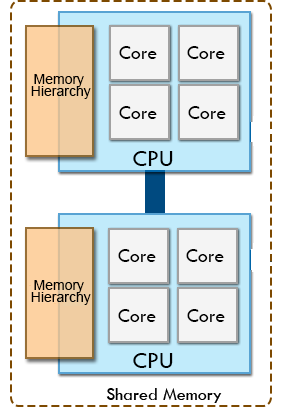
\includegraphics[scale=0.45]{imgs/homoplats.png}
		\caption{Schematic representation of a homogeneous system.}
		\label{fig:homoplat}
	\end{center}
\end{figure}

\subsubsection*{CPU devices}
\label{cpu_devices}

Gordon Moore predicted, in 1965, that for the following ten years the number of transistors on the CPU chips would double every 1.5 years \cite{MooreLaw}. This was later known as the Moore’s Law and it is expected to remain valid at least up to 2015. Initially, this allowed the increase in CPU chips clock frequency by the same factor as the transistors. Software developers did not spend much effort optimising their applications and only relied on the hardware improvements to make them faster.

Due to thermal dissipation issues, the clock frequencies of CPU chips started to stall in 2005. Manufacturers shifted from making CPUs faster to increasing their throughput by adding more cores to a single chip, reducing their energy consumption and operating temperature. This marked the beginning of the multicore and parallel computing era, where every new generation of CPUs get wider, while their clock frequencies remain steady.

CPU devices are designed as general purpose computing units, and may contain multiple cores, each based on a simple structure of small processing units with a very fast hierarchical memory attached (cache, whose purpose is to hide the high latency access to global memory), and all the necessary data load/store and control units. They are capable of delivering a good performance in a wide range of operations, from executing simple integer arithmetic to complex branching and SIMD (single instruction multiple data, later explained) instructions. A single CPU core implements various mechanisms for improving the performance of applications, at the hardware level, with the most important explained next:

\begin{center}
	\begin{description}
		\item[ILP] instruction level parallelism (ILP) is the overlapping of instructions, performed at both the hardware and software level, which otherwise would run sequentially. At the software level it is denominated as static parallelism, where compilers try to identify which instructions are independent, meaning that the outcome of one does not affect the execution of the other, and schedules them to be executed at the same time, if the hardware has resources to do so. At the hardware level, ILP can be referred as dynamic parallelism as the hardware dynamically identifies which instructions execution can be overlapped while the application is running.

		\item[Vector instructions] are a special set of instructions based on the SIMD model, where a single instruction is simultaneously applied to a set of data. CPU instruction sets offer special registers and instructions that allow to execute a operation on a chunk of data in a special arithmetic unit. One of the most common examples is addition of two vectors. The hardware is capable of adding a given number of elements of the vectors . This optimisation is often done at compile time.

		\item[Multithreading] is the hardware support for the execution of multiple threads in a CPU core. This is possible by replicating part of the CPU resources, such as registers, and can lead to a more efficient utilisation of the CPU core hardware. If one thread is waiting for data, other thread can resume execution while the former is stalled. It also allows a better usage of resources that would otherwise be idle during the execution of a single thread. If multiple threads are working on the same data, multithreading can reduce the synchronisation between them and lead to a better cache usage.
	\end{description}
\end{center}

\subsection{Heterogeneous Systems}
\label{hetero_systems}

With the emerging use of hardware specifically designed for some computing domains, denominated hardware accelerators, whose purpose is to efficiently solve a given problem, a new type of computing platform is becoming increasingly popular. This marked the beginning of heterogeneous systems, where one or more CPU devices, operating in a shared memory environment similar to homogeneous systems presented in subsection \ref{homo_systems}, are coupled with one or more hardware accelerators. In current heterogeneous systems, CPUs and accelerators operate in a distributed memory model, meaning that data must be explicitly passed from the CPU to the accelerator, and vice-versa.

\begin{figure}[!htp]
	\begin{center}
		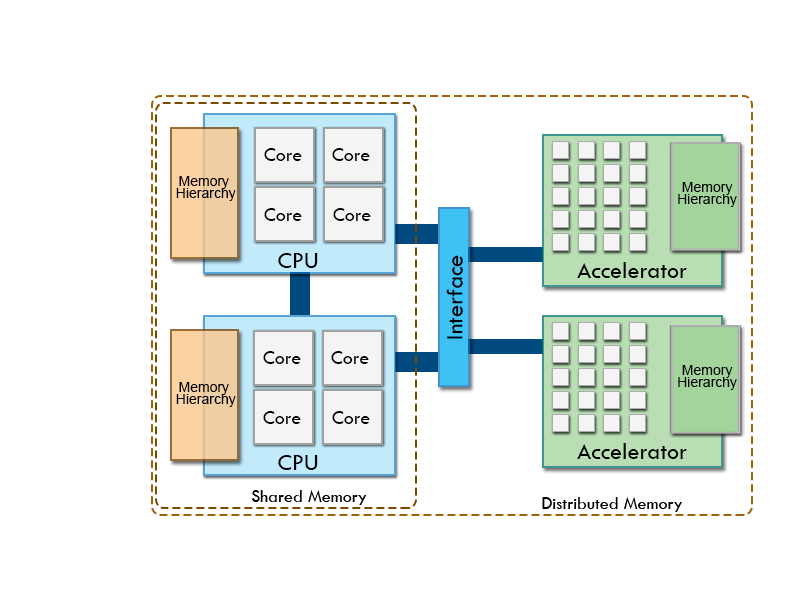
\includegraphics[scale=0.45]{imgs/heteroplats.png}
		\caption{Schematic representation of a heterogeneous system.}
		\label{fig:heteroplat}
	\end{center}
\end{figure}

Figure \ref{fig:heteroplat} presents a schematic representation of a heterogeneous system. Note that both CPUs must use the same interface to communicate with the hardware accelerators, which may cause contention. This high latency interface, PCI-Express being the most common, usually is a potential bottleneck for applications that use accelerators.

Computing accelerators are usually built with a large number of small and simple processing units, aimed to achieve the most performance possible on specific problem domains, as opposed to general purpose CPUs. They are oriented for massive data parallelism processing (SIMD architectures), where a single operation is performed on huge quantities of independent data, with the purpose of offloading the CPU from such data intensive operations. Several manycore accelerator devices are available, with me most popular being the general purpose GPUs to the Intel Many Integrated Core line, currently known as Intel Xeon Phi \cite{Intel:MIC}. An heterogeneous platform may have one or more accelerator devices of the same or different architectures.

As of November 2013, over 50 of the TOP500’s list \cite{TOP500} are computing systems with hardware accelerators, which indicates an exponential growth in usage compared to previous years. The Intel Xeon Phi is becoming increasingly popular, being the accelerator device of choice in 13 clusters of the TOP500, with one of them being the Tianhe-2 which is the faster system on the list. NVidia GPUs remain as the most used accelerator, with the AMD steadily losing their share.

\subsubsection*{Graphics Processing Unit}
\label{gpu}

The Graphics Processing Units (GPU) were one of the first hardware accelerators on the market. Their purpose is to accelerate computer graphics applications, which started of as simple pixel drawing and evolved to support complex 3D scene rendering, such as transforms, lighting, rasterisation, texturing, depth testing, and display. Due to the industry demand for customisable shaders, this hardware later allowed some flexibility for the programmers to modify the image synthesising process. This also allowed using this GPUs as a hardware accelerator for wider purposes beyond computer graphics, such as scientific computing, as some researchers saw the potential to use these devices to boost the performance of numerical computation.

The GPU architecture is based on the SIMD model. Its original purpose was to process and synthesise images, which are, from the computation point of view, a large set of numbers representing pixels. The processing of each pixel usually does not depend on the processing of its neighbours, or any other pixel on the image, so the computation has no data dependencies in the best case scenario. This allows to process all pixels simultaneously. The massive data parallelism is the most important characteristic that was considered when designing the GPU architecture.

As the GPU manufacturers allowed more flexibility to program their devices, the High Performance Computing (HPC) community started to use them to solve specific massively data parallel problems, such as numerical computation problems. However, the highly specialised architecture of GPUs affects the performance of many other problem domains. Due to the increased demand for these devices by the HPC community, manufacturers began to generalise more of the GPUs features, such as adding support for double precision floating point arithmetic, and later began producing accelerators specifically oriented for scientific computing. \nvidia is the number one GPU manufacturer for scientific computing GPUs, with a wide range of available hardware known as Tesla. These devices characteristics differ from the general purpose GPUs, as they have more GDDR RAM, a different structural design to fit in cluster nodes, and different cooling options. The chip itself is different, offering more processing units and larger caches. The latest architecture released by \nvidia is named Kepler \cite{NVIDIA:Kepler}, and its relevant architecture details are explained next.

\begin{figure}[!htp]
	\begin{center}
		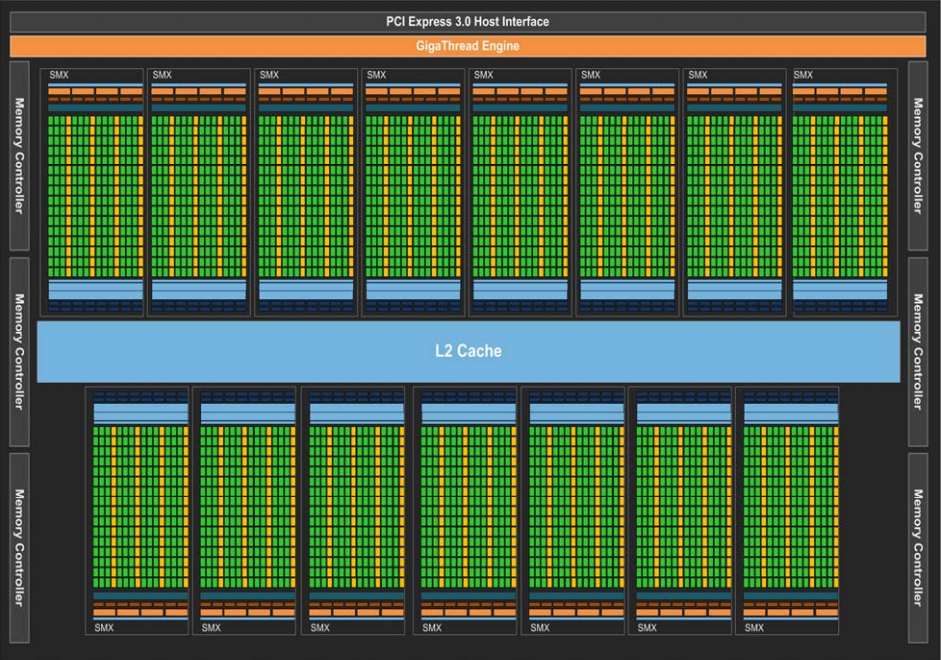
\includegraphics[scale=0.45]{imgs/kepler_arch.png}
		\caption{Schematic representation of the \nvidia Kepler architecture.}
		\label{fig:kepler}
	\end{center}
\end{figure}

As figure \ref{fig:kepler} shows, the Kepler architecture is organised into two main components: the Streaming Multiprocessor (SMX) and the memory module. The focus of this architecture was not only the performance but the energy efficiency, offering up to to 3x more performance per watt than Fermi (the previous architecture). In addition, the Kepler has implemented several features to improve the usage of resources:

\begin{description}
	\item[Dynamic Parallelism:] a kernel (algorithm coded to run on the GPU) on the GPU is capable of being called recursively, which allows to dynamically generate new load to process, without the CPU interfering. This allows for less regular algorithms to run on the GPU and reduces the communication between CPU and GPU as it is capable of managing the workload.
	\item[Hyper-Q:] this system increases the amount of work queues to 32 simultaneously hardware managed connections. With this, multiple CPU cores can launch new different kernels on the CPU at the same time, increasing the resource usage. Now, multiple threads of the same application are not required to have exclusive usage of the GPU, reducing the amount of synchronisations.
	\item[Grid Management Unit:] to allow for dynamic parallelism a new grid (a collection of threads of a kernel, later explained in more detail) management system is required. The new system also allows to schedule multiple grids, which allows for different kernels, from possibly different threads, to run simultaneously (Hyper-Q).
	\item[\nvidia GPUDirect:] this feature allows GPUs in a single system, or in a interconnected network, to share data without the interference of the CPU and system memory, creating a direct connection to Solid State Drives and other similar devices, and reducing the communication latency.
\end{description}

The SMX are the units responsible for performing all computations on the GPU, and a chip may have up to 15. Each SMX has 192 single precision and 64 double precision CUDA cores, small processing units capable of performing basic arithmetic, 32 special function units, to perform complex computations such as trigonometric operations, and 32 load and store units. These computing units operate at the GPU main clock rate. The SMX features 4 warp schedulers (warps are explained next) and 8 instruction dispatchers.

Memory wise, each SMX has 65536 32-bit registers, with a maximum of 255 registers per CUDA thread, a 64 KByte very fast memory for L1 cache and shared memory, and a similar fast 48 KByte memory cache for read-only data. Finally, the Kepler architecture provides 1536 KB of L2 cache shared among all SMX units. The high end available Tesla K40 has a memory bandwidth of 280 GB/s to its main memory. Since the GPU is connected by PCI-Express interface, the bandwidth for communications between CPU and GPU is restricted to only 12 GB/s (6 GB/s in each direction of the channel). Memory transfers between the CPU and GPU must be minimal as it greatly restricts the performance.

A kernel is executed by a given amount of parallel workers named CUDA threads. They are grouped into blocks, to be scheduled among SMX and the threads inside a block can only run in a given SMX, and these are grouped into a grid, which contains all CUDA threads (up to $2^{31}-1$) for a given kernel. The CUDA threads are grouped in batches of 32, called warps, to be dispatched by a warp scheduler. The scheduler has a scoreboard with up to 48 entries to manage which warps are stalled waiting for resources or data and which are ready to be executed.

\subsubsection*{Intel Many Integrated Core architecture}
\label{mic}

The \intel Many Integrated Core (MIC) architecture, with the current production device known as \intel Xeon Phi, is an emerging technology becoming adopted by various clusters in the TOP500 list. It has a design different from the \nvidia GPUs presented previously, opting to have fewer computing units but capable of performing more complex operations. Figure \ref{fig:mic} presents a schematic representation of the architecture. The current high end model, the \intel Xeon Phi 7120p, has 61 cores and 16 GB GDDR5 RAM. The device has three operating modes:

\begin{description}
	\item[Native:] the device acts as an independent system itself, with one core reserved for the operating system execution. The application and all libraries must be compiled specifically to run on the device, and later copied to the its memory along with the necessary input data, prior to its execution. No further interaction with the CPU is required until the application has executed.
	\item[Offload:] the device acts an accelerator, such as a GPU. Only part of the application is set to run on the Xeon Phi, and data must be explicitly passed between CPU and device as required by the code that it will compute. All library functions called inside the device must be specifically compiled for it. Note that it is not possible to have an entire library compiled for the Xeon Phi and CPU simultaneously.
	\item[Message passing:] the device acts as an individual computing system in the network. Memory transfers are explicitly and the device can be programmed using the Message Passing Interface (MPI) \cite{MPI}. The restrictions mentioned in the previous point are also applicable.
\end{description}

\begin{figure}[!htp]
	\begin{center}
		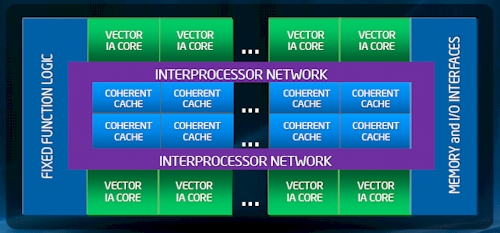
\includegraphics[scale=0.65]{imgs/mic.png}
		\caption{Schematic representation of the \intel Many Integrated Core architecture.}
		\label{fig:mic}
	\end{center}
\end{figure}

Each core is able to run 4 threads simultaneously, and most of the massive parallelism is obtained by he 32 512 bit wide vector registers available. The core as 64 KB for data and 64 KB for instruction L1 cache, and 512 KB L2 cache. There is no shared cache among the 61 cores of the chip, and no cache consistency and coherence is automatically guaranteed among them. The cores are interconnected by a bidirectional ring network. MIC does not support out of order execution, which greatly compromises the use of ILP. Also, the clock frequency is limited to 1.33 GHz, which is less than half of the modern CPUs.

Since it uses the same instruction set as conventional x86 CPUs, \intel claims that current applications can be easily ported to run on the device. This may be true for common matrix arithmetic and similar applications, efficient ports of complex applications that require the use of many external libraries is very difficult, or even infeasible \cite{Msc:AMP}.

\subsubsection*{Other hardware accelerators}
\label{other_accelerators}

More hardware accelerators are coming to the market due to the increasingly popularity of GPUs and Intel MIC among the HPC community. Texas Instruments developed their new line of Digital Signal Processors, best suited for general purpose computing while very power efficient. Their capable of delivering 500 GFlop/s (giga floating point operations per second), consuming only 50 Watts \cite{Texas:DSP}.

ARM processors are now leading the mobile industry and, alongside the new NVidia Tegra processors \cite{NVIDIA:Tegra} that are steadily increasing the market share, are likely to be adopted by the HPC community\footnote{e.g. the ARM based Montblanc project will replace the MareNostrum in the Barcelona Supercomputing Center (BSC)} due to their low power consumption while delivering a significant performance \cite{ARM}. Due to the increased complexity of mobile applications, the shift from 32 bit to 64 bit mobile processors has already happened, which will greatly benefit computing clusters using this type of hardware.

\section{Software}
\label{software}

Most programmers (both computer scientists and self-taught programmers) are only used to code and design sequential applications, showing a lack of know-how to develop algorithms for parallel environments. This lack of expertise is even greater when programming for heterogeneous systems, where programming paradigms shift when considering different hardware accelerators. The mainstream industry is still adopting the use of multicore architectures with the purpose of increasing their processing power, reflecting in a lack in the academic training of computer scientists on code optimisation and parallel programming. Self taught programmers have an increased obstacle due to the lack of theoretical basis when using these new parallel programming paradigms.

Programming for multicore environments requires some knowledge of the underlying architectural concepts of CPU devices and how they are interconnected. Shared memory, cache coherence and consistency and data races are architecture-specific aspects that the programmer does not face in sequential execution environments. However, these concepts are fundamental not only to ensure efficient use of the computational resources, but most importantly the correctness of the application.

Heterogeneous systems combine the flexibility of multicore CPUs with the specific capabilities of manycore accelerator devices. However, most computational algorithms and applications are designed with the specific characteristics of CPUs in mind. Even multithreaded applications usually cannot be easily ported to these devices expecting high performance. To optimise the code for these devices it is necessary a deep understanding of the architectural principles behind their design.

The workload balance between the cores of a single CPU chip is an important aspect to extract performance and get the most efficient usage of the available resources. A inadequate workload distribution may cause some cores of the CPU to be starved, unnecessarily increasing the application execution time. A good load balancing strategy ensures that all the cores are used as most as possible. Considering a multi-CPU system, it is important to manage the data in such a way that it is available in the memory bank of the CPU that will need it to avoid the NUMA latency. The same concepts apply when balancing the load between CPU and hardware accelerators, with the increased complexity of the distributed memory environment and high latency data transfers.

Some computer science groups developed libraries that attempt to abstract the programmer from specific architectural and implementation details of these systems, providing an easy API as similar as possible to current sequential programming paradigms. The next subsections will present frameworks to aid the development of parallel applications for homogeneous and heterogeneous systems.

\subsection{Shared Memory Environments}
\label{shared_mem}

Homogeneous systems often operate in a shared memory environment. Using multiple CPU devices may cause the memory banks to be physically divided but hardware mechanisms, such as specialised CPU interconnections, allow for a common addressing space. Libraries and frameworks for parallelising for this environment are presented next.

\subsubsection*{pThreads}

Threads are the most simple parallel task that can be scheduled by the operating system. POSIX Threads (pThreads) are the standard implementation for UNIX based operating systems with POSIX conformity, such as most Linux distributions and Mac OS. The pThreads API provides the user with primitive for thread management and synchronisation. Since this API forces the user to deal with several low level implementation details, such as data races and deadlocks, the industry demanded the development of high abstraction level libraries, which are usually based on pThreads.

\subsubsection*{OpenMP, TBB, and Cilk}

OpenMP \cite{OpenMP}, Intel Threading Building Blocks (TBB) \cite{Intel:TBB}, and Cilk \cite{Intel:Cilk} are the most popular high level libraries for parallel programming in homogeneous systems.

The OpenMP API is designed for multi-platform shared memory parallel programming in C, C++, and Fortran, for all available CPU architectures. It is portable and scalable, and aims to provide a simple and flexible interface for developing parallel applications, even for the most inexperienced programmers. It is based in a work sharing strategy, where a master thread spawns a set of slave threads and compute a task in a shared data structure.

Intel TBB employs a work stealing heuristic, where, after the initial load distribution, if the task queue is empty a thread attempts to steal a task from other busy threads. It provides a scalable parallel programming task based library for C++, independent from architectural details, and only requires a C++ compiler. It automatically manages the load balancing and some cache optimisations, while offering parallel constructors and synchronisation primitives for the programmer. However, it requires knowledge of the object oriented programming paradigm.

Cilk is a runtime system for multithreaded programming in C++. It maintains a stack with the remaining work, employing a work stealing heuristic similar to the Intel TBB.

\subsection{Distributed Memory Environments}
\label{distributed_mem}

Heterogeneous systems use distributed memory address space for handling the data between CPU and accelerator devices. Even though the CPU devices work on a shared memory space, data must be explicitly passed to the accelerators. General purpose frameworks for parallelising on the devices and on the heterogeneous platforms as a whole are presented next.

\subsubsection*{Message Passing Interface}

The Message Passing Interface (MPI) \cite{MPI}, designed by a consortium of both academic and industry researchers, has the objective of providing a simple API for process based parallel programming in distributed memory environments. It relies on point-to-point and group messaging communication, and is available in Fortran and C. It is often used in conjunction with a shared memory parallel programming API, such as OpenMP, for work sharing between computing nodes, with the latter ensuring a more efficient parallelisation inside each node.

Intel adapted an MPI version to work on both their CPUs and Xeon Phi, considering the device as a set of CPUs. Communications between the CPU and the device are explicitly handled by the programmer by calling specific functions. The other alternative to program for this device with MPI is to use compiler \textit{pragma} directives for data communication and code parallelisation.

\subsubsection*{CUDA}

The Compute Unified Device Architecture (CUDA) is a computing model for hardware accelerators launched in 2007 by \nvidia and aims to provide a framework for programming devices similar architecture to the \nvidia GPUs. It has a specific instruction set architecture (ISA) and allows programmers to use GPUs for scientific computing.

\nvidia considers that a parallel task is constituted by a set of CUDA threads, which execute the same instructions coded in the kernel (conditional jumps are a special case that will be later explained) but on different data. Considering the sum of two vectors, each CUDA thread will be responsible for adding a single element of the vectors.

The CUDA thread is the most basic data independent parallel task, which can run simultaneously with other CUDA threads, and it is organised in a hierarchy presented in figure \ref{fig:cuda}. A block is a set of CUDA threads that is matched by the global scheduler to run on a specific SMX. A grid is a set of blocks, representing the whole parallel kernel. Note that both the blocks and the grid sizes must be defined by the programmer, according to the algorithm, before calling the kernel, within the maximum values allowed by the GPU architecture.

\begin{figure}[!htp]
	\begin{center}
		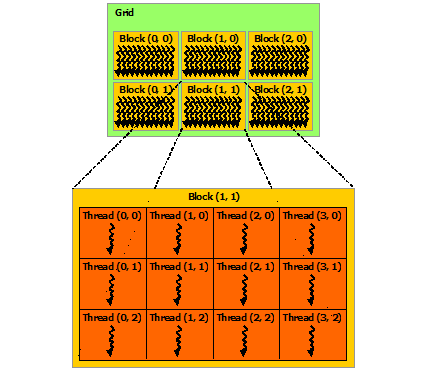
\includegraphics[scale=0.9]{imgs/cuda_threads.png}
		\caption{Schematic representation of CUDA thread hierarchy.}
		\label{fig:cuda}
	\end{center}
\end{figure}

Conditional jumps must be avoided as they may cause different CUDA threads within the same warp execute different instructions. Since inside an SMX it is not possible to have 2 threads simultaneously executing different instructions, the divergent branches will be executed sequentially, doubling the warp execution time.

\subsubsection*{DICE}

The DICE framework aims to provide the tools to help building efficient and scalable applications for heterogeneous platforms, with accelerator devices that support CUDA. It creates an abstraction layer between the architectural details of heterogeneous platforms and the programmer, aiding the development of portable and scalable parallel applications. Its main focus is to obtain the best performance possible on irregular applications, rather than abstracting all the architecture details from the programmer. The programmer still needs to have some knowledge of each different architecture and programming paradigms, and he needs to instruct the framework about how tasks should be divided in order to fit the requirements of the different devices. 

Instead of relying in pre-partitioned work, the programmer defines a function for dicing the dataset and the framework creates different sized chunks of data to distribute among the CPU and GPUs. Apart from this, the framework frees the programmer from managing the workload distribution, memory usage and data transfers between the available devices, but requires that the application is built according to the strict specifications of the framework. The programmer is able to tune specific details related to the memory transfers and load balance, if he is comfortable enough with the framework.

The scheduler uses the statistics provided by each job (a kernel set to run on a device) to adjust the scheduling policy and the granularity of the tasks. This dynamic granularity management allows to better suit the uneven execution times of irregular jobs. DICE uses a variant of the Heterogeneous Earliest Finish Time (HEFT) scheduling algorithm \cite{HEFT}, which uses the computation and communication costs of each task, in order to assign every task to a device in such a way that minimizes the estimated finish time of the overall task pool. This variant of HEFT attempts to make a decision every time it is applied to the task pool, so that tasks on the multiple devices take the shortest possible time to execute \cite{Msc:Mariano}.

DICE assumes a hierarchy composed of multiple devices (both CPUs and GPUs, in its terminology), where each device has access to a private address space (shared within that device), and a distributed memory system between devices. To abstract this distributed memory model, the framework offers a global address space. However, since the communication between different devices is expensive, DICE uses a relaxed memory consistency model, where the programmer can use a synchronisation primitive to enforce memory consistency. DICE implements a shared software cache so that every device has the data as close as possible, using the local memory of each device. It also ensures that each device has a copy of a given data partition, which otherwise would only be stored in the CPU memory.

\subsubsection*{StarPU}

StarPU \cite{STARPU} is a unified runtime system consisting on both compiler directives and a runtime API that aims to allow programmers to efficiently extract parallelism from heterogeneous platforms by abstracting the architecture details of these systems. This framework frees the programmer of the workload scheduling and data consistency inherent from the distributed memory environment of heterogeneous platforms. Task submissions are handled by the StarPU task scheduler, and data consistency is ensured via a data management library.

However, one of the main differences to DICE is that StarPU attempts to increase performance by carefully considering and attempting to reduce memory transfer costs. This is done using history information for each task and, accordingly to the scheduler decision of where a task shall be executed, asynchronously prepare data dependencies, while the system is busy computing other tasks. The task scheduler itself can take this into account, and determine where a task should be executed by taking into account not only the execution history, but also the estimation of data transfers latency.

StarPU employs a task based approach to the programming model, where a kernel is considered a parallel task. Based on the scheduler and available implementations for the kernel (i.e., can only run on CPU, GPU, or both), the framework handles where and how much load each task will compute. It provides a set of different schedulers for the programmer to chose.

The performance model differs from the schedulers implemented in StarPU, but most resort to a history of the tasks execution on the devices. All the schedulers use a user defined calibration to start the execution, and after 10 executions of each task it starts to perform a real-time calibration with the available statistics. This may translate in a not efficient usage of the system resources at the start of the application, but ensures that it tends to improve as the application runs.

The memory consistency is automatically ensured by the framework, as it transfers the data asynchronously without the programmer interaction. The data dependencies are determined by the scheduler, with some interaction of the programmer, as he must declare if a data structure is read/write or both. The granularity of the tasks must be defined by the user, as opposed to the DICE dynamic adjustment.

\subsubsection*{OpenACC}

OpenACC \cite{OpenACC} is a framework for heterogeneous platforms with accelerator devices. It is designed to simplify the programming paradigm for CPU/GPU systems by abstracting the memory management, kernel creation, and GPU management. Like OpenMP, it is designed for C, C++ and Fortran, it provides both an API and compiler directives, and allows the parallel task to run on both CPU and GPU at the same time. However, it does not schedule the load between the CPU and GPU. The current specification addresses both \nvidia and AMD GPUs, as well as the \intel Xeon Phi.

However, this framework offers more of an abstraction of the hardware accelerator used, focusing on portability across heterogeneous platforms, rather than abstracting the intrinsic complexities of these systems.

\subsubsection*{OpenHMPP}

OpenHMPP \cite{OpenHMPP} is a standard similar to OpenACC, developed by CAPS \cite{CAPS} to develop parallel applications for heterogeneous platforms. It attempts to abstract the complexities of GPU accelerators by providing a set of compiler directives for efficient parallelisation. In the current specification, OpenHMPP uses a superset of the OpenACC directives for offloading code to the GPU and managing the data transfers, in both C and Fortran.

Although it provides asynchronous execution of the offloaded kernel, it is not possible to use these framework to manage simultaneous execution and load balance of the same kernel in both CPUs and GPUs. Moreover, it is only possible to use this specification with the CAPS compilers and PathScale ENZO Compiler Suite \cite{ENZO}.

\subsection{Particle Physics Frameworks}
\label{particle_frameworks}

\subsubsection*{ROOT}

ROOT \cite{CERN:ROOT} is a very complex framework coded by physicists to aid all data analysis application development of the physics experiments conducted at CERN. It has all functionality required to process large amounts of data, by providing specific data storage formats, C++ classes for elemental particles, various physics algorithms, and histogram creation functions. The framework also provides a built-in C++ interpreter, Cling, to allow testing simple instructions and macros, without the need to compile and link the code.

PROOF is a subset of the framework to support the development of data analysis applications in distributed memory environments. However, it is only designed to work with a set of computing nodes, with a master/slave process hierarchy, without support for hardware accelerators. Also, it does not focus on the efficient usage of the available computational resources, only distributes the load on demand among the processes.

Currently, ROOT does not provide parallel functionalities, specially for shared memory environments, but the developers already shown interest to improve the performance of some core routines of the framework. However, it may not translate in massive performance gains of the data analysis applications, as the critical region is usually on the reconstruction of the events, which does not heavily rely on a small set of ROOT functionalities, but rather on a large set of non-complex routines and classes.

\subsubsection*{TopROOTCore}

TopROOTCore is an extension of ROOT for top quark physics, developed by CERN associate research groups,that adds more functionalities and physics algorithms to the existing framework. It is responsible for producing the last input data format at the last CERN computational tiers, before the final analysis and event reconstruction. In the data analysis applications, it is often used due to some physics algorithms it implements.

\subsection{Profiling Tools and Libraries}
\label{tools}

\subsubsection*{Performance API}

The Performance API (PAPI) \cite{PAPI} specifies an API to access hardware performance counters in most modern processors. It allows programmers to measure the performance counters for specific regions of an application, evaluating metrics such as cache misses, operational intensity or even power consumption. This analysis helps classifying the algorithms and identify possible bottlenecks at a very low abstraction level.

PAPI recently supports hardware counters for both \nvidia GPUs, trough the \nvidia CUPTI interface, and \intel Xeon Phi. It also supports counters to measure the energy efficiency of the hardware.

\subsubsection*{\nvidia CUPTI}

The \nvidia CUDA Profiling Tools Interface (CUPTI) \cite{NVIDIA:CUPTI} is a performance analysis interface available through the \nvidia drivers for CUDA capable GPUs. It provides a callback API to integrate with the code, at the entry and exit of a kernel call, which monitors the interaction of the code with the CUDA runtime and drivers. CUPTI has a second API to monitor the performance of a kernel on the GPU by analysing the hardware counters on the device, which allows for a in-depth assessment of the code behaviour in memory transactions, cache accesses and misses, and much more.

\subsubsection*{TAU and HPCToolkit}

TAU \cite{TAU} and HPCToolkit \cite{HPCToolkit} are performance analysis tools, with static and dynamic functionalities, to evaluate the performance of HPC applications. The static APIs are low level and, while providing higher control of the areas to profile and specific metrics, require the programmer a deeper knowledge of these tools and how to integrate them with the existing code. The dynamic functionalities provide more general metrics and do not require any changes to the application code.

Both tools provide statistical visualisation GUIs, to build graphs and comparisons of the different metrics profiled during the application execution time. Note that both tools support the analysis of parallel code in both shared and distributed memory environments, but the HPCToolkit still does not support any hardware accelerator. Unlike VTune, these tools only present the statistics but do not attempt to identify the bottlenecks, leaving that task to the programmer.

\subsubsection*{VTune}

Intel VTune profiler \cite{Intel:VTune} is a proprietary tool for performance analysis of applications. It provides an easy to use interface to analyse applications, automatically identifying its bottlenecks, without any change to the source code. It intercepts the system calls to assess the execution time and behaviour, such as efficient cache usage, of the routines of an application. VTune also provides visualisation functionalities to make the profiling of parallel applications a simple task for developers with small experience. It works with both \intel and GNU compilers.

\subsubsection*{VampirTrace}

VmpirTrace \cite{VampirTrace} is a open source library to analyse an application execution on both shared memory and distributed memory environments, with support for CUDA capable GPUs through the CUPTI interface. It is capable of analysing the CPU hardware counters per thread/process by resorting to the Performance API. It has a low level API to integrate with the code to measure specific metrics and regions of the code, and a more abstract interface that allows tracing the application execution without the need to change the code.

Additionally to other similar tools, VampirTrace allows to analyse the I/O interactions of an application, such as access times, types, and patterns to the hard drives.

\subsubsection*{\nvidia Nsight}

The \nvidia Nsight \cite{NVIDIA:Nsight} is a developer more of a platform rather than a framework for heterogeneous computing. It is available for both Visual Studio and Eclipse and aids the development of code for CUDA capable GPUs, with easy integration with current official production libraries. It has real time debugging functionalities to test code running on both CPU and GPU simultaneously. The built-in profiler allows to perform analysis to the kernels execution time on GPU, load and store efficiency (related to the coalesced accesses of CUDA threads to memory), SMX occupancy rate, and memory usage. The profiling metrics are the same as the ones provided by the Performance API, as they both use the \nvidia CUPTI interface.
